\chapter{Paquímetro}\label{paquimetro}

\vspace{-0.5cm}


O paquímetro é um instrumento utilizado para medir dimensões de objetos relativamente pequenos, desde uns poucos centímetros até frações de milímetros, com uma precisão da ordem do centésimo de milímetro. Este instrumento é delicado e deve ser manipulado com cuidado e precaução. 

Ele é formado por uma régua com um esquadro num extremo, sobre a qual se desliza o outro esquadro destinado a indicar o valor medido sobre a escala.  Sobre o esquadro móvel encontra-se o nônio que possui uma segunda escala dedicada a marcar as subdivisões do milímetro. Na Figura~\ref{fig:p1} podemos ver um desenho de um paquímetro típico.

\begin{figure}[h]
\begin{center}
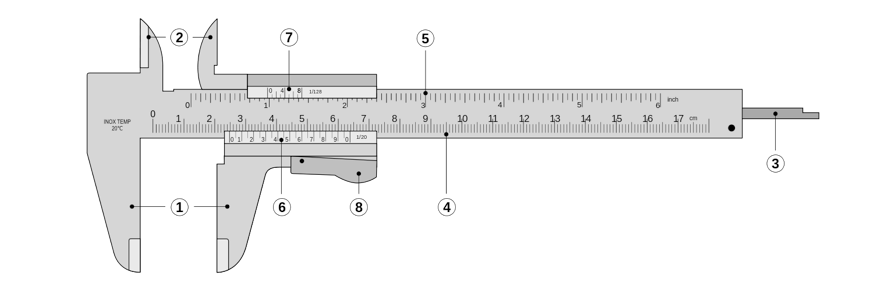
\includegraphics[width=14cm]{fig/Paquimetro1}
\caption{\label{fig:p1} Paquímetro formado por: \textcircled{1} Encostos para medidas externas; \textcircled{2} Orelhas para medidas internas; \textcircled{3} Haste de profundidade; \textcircled{4} Escala principal inferior (graduada em centímetros e milímetros); \textcircled{5} Escala principal superior (graduada em polegadas e frações de polegadas); \textcircled{6} Nônio ou vernier para leitura das frações de milímetros em que esteja dividido; \textcircled{7} Nônio ou vernier para leitura das frações de polegada em que esteja dividido; \textcircled{8} Propulsor e trava.}
\vspace{-0.5cm}
\end{center}
\end{figure}

Para utilizar o paquímetro, primeiramente se separam os encostos para que o objeto a ser medido possa ser colocado entre eles, logo se fecham estes encostos de forma que o objeto fique preso ao mesmo e se bloqueia o movimento do esquadro móvel para poder realizar a leitura do valor medido. Usaremos o exemplo mostrado na Figura~\ref{fig:p2} para facilitar a explicação de como fazer a leitura. 

\begin{figure}[h]
\begin{center}
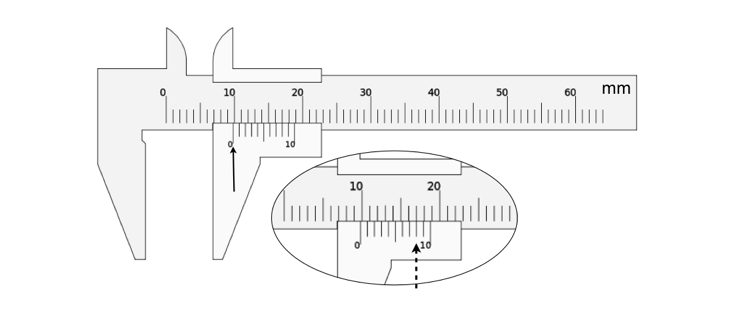
\includegraphics[width=14cm]{fig/Paquimetro2}
\caption{\label{fig:p2} Exemplo de uma medição realizada com paquímetro graduado em mm e com um nônio com 10 divisões. Valor medido (0,98 $\pm$ 0,01) cm. Ver texto.}
\vspace{-0.5cm}
\end{center}
\end{figure}

O primeiro passo é fazer a leitura sobre a escala principal (Figura~\ref{fig:p1}) e para isso observamos a posição do zero do nônio, que no exemplo está levemente deslocada à direita dos 9 mm (seta cheia na figura~\ref{fig:p2}). Desta forma temos a primeira parte da medida, sendo 0,9 cm. Vemos que as seguintes marcas do nônio também estão levemente deslocadas à direita e que esta diferença vai se reduzindo paulatinamente. Verificamos que a oitava marcação sobre o nônio coincide com a marcação com a régua principal (seta tracejada na Figura~\ref{fig:p2}) e logo as marcas do nônio vão ficando progressivamente à esquerda das marcas da régua fixa. Portanto a segunda parte da leitura nos diz que o valor medido é de 0,98 cm com uma incerteza de 0,01 cm.  Para a determinação da incerteza, considerada aqui como a mínima divisão do instrumento, temos que determinar o número de subdivisões do milímetro dado pelo nônio.  No caso do exemplo, temos 10 subdivisões, sendo a incerteza 1 mm dividido 10, ou seja 0,1 mm.  Finalmente o resultado da medição é: (0,98 $\pm$ 0,01) cm.

\underline {Importante:} Lembrar de verificar que o paquímetro esteja corretamente calibrado, ou seja que quando não haja abertura dos dois encostos, o zero da escala principal e do nônio sejam coincidentes.  

Mais informações sobre o uso do paquímetro podem ser encontradas na página  \url{http://www.stefanelli.eng.br/webpage/metrologia/p-nonio-milimetro-05.html}.